\pagestyle{MyStyle}

\chapter[Connectome-based patterns of first-episode medication-naïve patients with schizophrenia]{Connectome-based patterns of first-episode medication-naïve patients with \\schizophrenia}

\chaptermark{Connectome in first-episode medication-naïve schizophrenia}

\label{ch:rcscz}

\begin{refsection}

\begin{flushright}
\textit{Long-Biao Cui \textsuperscript{1}, Yongbin Wei \textsuperscript{1}, Yi-Bin Xi, Alessandra Griffa, Siemon C. de Lange, René S. Kahn, Hong Yin, Martijn P. van den Heuvel}\\
Schizophrenia Bulletin, 2019, sbz014

\vspace{5 mm}

\textsuperscript{1} these authors contributed equally to this work\\

\vspace{7 mm}

\end{flushright}

\newpage
\section*{Abstract}
Emerging evidence indicates that a disruption in brain network organization may play an important role in the pathophysiology of schizophrenia. The neuroimaging fingerprint reflecting the pathophysiology of first-episode schizophrenia remains to be identified. Here, we aimed at characterizing the connectome organization of first-episode medication-na\"{i}ve patients with schizophrenia. A cross-sectional structural and functional neuroimaging study using two independent samples (principal dataset including 42 medication-na\"{i}ve, previously untreated patients and 48 healthy controls; replication dataset including 39 first-episode patients [10 untreated patients] and 66 healthy controls) was performed. Brain network architecture was assessed by means of white matter fiber integrity measures derived from diffusion-weighted imaging (DWI) and by means of structural-functional (SC-FC) coupling measured by combining DWI and resting-state functional magnetic resonance imaging. Connectome rich club organization was found to be significantly disrupted in medication-na\"{i}ve patients as compared with healthy controls (\pval = 0.012, uncorrected), with rich club connection strength (\pval = 0.032, uncorrected) and SC-FC coupling (\pval < 0.001, corrected for false discovery rate) decreased in patients. Similar results were found in the replication dataset. Our findings suggest that a disruption of rich club organization and functional dynamics may reflect an early feature of schizophrenia pathophysiology. These findings add to our understanding of the neuropathological mechanisms of schizophrenia and provide new insights into the early stages of the disorder.

\section*{Introduction}
Recent analyses of brain structure \citep{Brugger2017HeterogeneityAH,Dietsche2017StructuralBC} and function \citep{Dong2018DysfunctionOL} have indicated that disruptions in brain network organization may play an important role in schizophrenia. These findings suggest that the disorder may involve a deficit of neural communication efficacy and information integration in the brain's connectivity network \citep{vanDenHeuvel2010AberrantFA}.

A network attribute of particular interest in the investigation of schizophrenia is the brain's "rich club" \citep{vanDenHeuvel2011RichclubOO}.  The rich club describes a set of densely connected hub regions, suggested to provide an anatomical backbone for functional information communication and integration \citep{Abraham2017DerivingRB,vanDenHeuvel2012HighcostHB}. Network studies have suggested that chronic schizophrenia is characterized by an abnormal rich club organization, with reduced brain connectivity among hub regions \citep{vanDenHeuvel2013AbnormalRC}. Studies have reported rich club abnormalities in schizophrenia and psychosis patients \citep{Yeo2016GraphMO,Klauser2017WhiteMD,Crossley2017ConnectomicCO}, as well as in subjects at high risk for the disorder \citep{Collin2014ImpairedRC} and general psychosis \citep{Schmidt2017StructuralND}, suggesting that rich club disorganization may be a central aspect of the neurobiological background of psychotic disorders.

One of the obstacles in identifying neuroimaging markers of schizophrenia pathophysiology is the clinical heterogeneity inherent to the nature of the disorder \citep{Millan2016AlteringTC}, underscoring the importance of minimizing confounding factors such as prior therapeutic exposure and the potential influence of chronicity. An important step in the investigation of neuroimaging signatures of schizophrenia is thus to study first-episode, medication-na\"{i}ve patients whose medical history is short and therapy is absent. Here, we examined the connectome structure in first-episode (with the majority medication-na\"{i}ve) schizophrenia patients using diffusion-weighted imaging (DWI) and resting-state functional magnetic resonance imaging (rs-fMRI).

\section*{Methods}
\subsection*{Participants}
Two independent datasets of first-episode schizophrenia patients were recruited at the Department of Psychiatry, Xijing Hospital. This study was approved by the local ethics committee and all participants (or their parents for those under age of 18 years) gave written informed consent after a full description of the aims and design of the study. Table 1 and the Supplementary Methods provide further details on the two datasets.

The resulting principal dataset included 42 patients with first-episode schizophrenia (all untreated, medication-na\"{i}ve patients, table 1) and 48 controls \citep{Cui2017AberrantPA,Cui2018DiseaseDF}. The structural clinical interview for Diagnostic and Statistical Manual of Mental Disorders, Fourth Edition, Text Revision (DSM-IV-TR) was used, and consensus diagnoses were made using the available data by 2 senior psychiatrists. Each patient was assessed at the time of scanning using the Positive and Negative Syndrome Scale (PANSS).

The replication dataset included 39 first-episode patients with schizophrenia. This set included 10 untreated, medication-na\"{i}ve patients, 29 patients with no more than 2 weeks of cumulative exposure to antipsychotics (see Table \ref{table1:demongraphics}), and 66 age- and gender-matched controls. Neuroimaging data of the control subjects have been investigated in a prior study \citep{Cui2018DiseaseDF}. Patients were diagnosed according to the DSM, Fifth Edition (DSM-5) and assessed at the time of imaging using the PANSS. In the main text, we report results obtained for the 10 untreated, medication na\"{i}ve patients. Results relative to the whole replication dataset of 39 patients are reported in the supplementary results.

\begin{sidewaystable}
\renewcommand{\arraystretch}{0.8}
\centering
\small
\fontfamily{phv}\selectfont
\captionof{table}{Demographical and Clinical Data of Participants}
\begin{tabular}{@{}llllclllclll@{}}\toprule
& \multicolumn{3}{c}{Principal Dataset} & \phantom{abc}& \multicolumn{3}{c}{Replication Dataset} \\
\cmidrule{2-4} \cmidrule{6-8}
& Patients & HCs &  && Patients & HCs &  \\
& (\textit{n}=42) & (\textit{n}=48) & \pval-values && (\textit{n}=39) & (\textit{n}=66) & \pval-values \\
\midrule
Sociodemographic\\
Age, years & 25.0 $\pm$ 6.4 & 26.3 $\pm$ 4.1 & 0.24\textsuperscript{a} && 24.6 $\pm$ 6.6 & 26.7 $\pm$ 5.6 & 0.09\textsuperscript{a} \\
Gender, male/female & 24/18 & 22/26 & 0.28\textsuperscript{b} && 21/18 & 39/27 & 0.60\textsuperscript{b} \\
Ethnicity, Han/others & 42/0 & 48/0 &  && 39/0 & 66/0 &  \\
Education level, year & 13.3 $\pm$ 1.7 & 14.5 $\pm$ 2.0 & 0.004\textsuperscript{c} && 11.9 $\pm$ 3.3 & 16.0 $\pm$ 3.4 & <0.001\textsuperscript{c} \\
Clinical\\
Inpatients/outpatients & 41/1 & - & && 37/2 & - & \\
Duration of illness, month\textsuperscript{d} & 11.3 $\pm$ 14.6 & - & && 13.7 $\pm$ 23.8 & - & \\
PANSS total score & 97.0 $\pm$ 18.5 & - & && 84.1 $\pm$ 12.0 & - & \\
PANSS positive score & 24.1 $\pm$ 8.3 & - & && 22.0 $\pm$ 4.7 & - & \\
PANSS negative score & 23.5 $\pm$ 8.3 & - & && 19.2 $\pm$ 6.1 & - & \\
PANSS general psychopathology score & 49.5 $\pm$ 8.9 & - & && 42.8 $\pm$ 7.3 & - & \\
Medical \\
Medication, no/yes & 42/0 & - & && 10/29 & - & \\
Risperidone & - & - & && 16 & - & \\
Risperidone and paliperidone & - & - & && 1 & - & \\
Risperidone and haloperidol & - & - & && 1 & - &\\
Risperidone adn clozapine & - & - & && 1 & - & \\
Olanzapine & - & - & && 7 & - & \\
Paliperidone & - & - & && 2 & - & \\
Amisulpride & - & - & && 1 & - & \\
Duration of treatment, day & - & - & && 4.3 $\pm$ 4.5 & - & \\
Dose equivalent, mg/day\textsuperscript{e} & - & - & && 5.5 $\pm$ 5.0 & - & \\
\bottomrule
\end{tabular}
\begin{flushleft}
\footnotesize
Note: HCs, healthy controls; NA, not applicable; PANSS, Positive and Negative Syndrome Scale. \textsuperscript{a} Two sample t-test. \textsuperscript{b} Chi-square test. \textsuperscript{c} Wilcoxon Rank Sum test was performed due to the non-normal distribution of samples. The medians of education years were statistically different between two groups. \textsuperscript{d} Duration of illness was determined from onset of disease until first meeting diagnosis. \textsuperscript{e} Antipsychotic dose equivalent to olanzapine based on defined daily doses method (WHO Collaborating Centre for Drug Statistics Methodology, 2014).
\end{flushleft}
\label{table1:demongraphics}
\end{sidewaystable}

\subsection*{Image acquisition and preprocessing}
High-resolution T1-weighted MRI, DWI, and rs-fMRI data were obtained for both cohorts. Specific scanning parameters are shown in supplementary tables. Data preprocessing steps \citep{vanDenHeuvel2013AbnormalRC} included parcellation of the cortex into 68 regions according to the Desikan-Killiany atlas \citep{DESIKAN2006968} by applying the FreeSurfer (version 5.3.0) pipeline (https://surfer.nmr.mgh.harvard.edu) on the T1-weighted images. Analyses based on 114 and 219 region parcellations \citep{CAMMOUN2012386} showed similar results (see supplementary results). White matter fiber tracts were reconstructed from DWI images using the following procedure \citep{VANDENHEUVEL2016293}. The 64 diffusion-weighted volumes (b = 1000 s/mm$^{2}$) and the obtained b = 0 volume were realigned and corrected for small head movements and gradient-induced distortions \citep{ANDERSSON2002177}. The diffusion profile within each voxel was reconstructed using generalized q-sampling imaging (GQI) \citep{YEH2010}, and fractional anisotropy (FA) maps were computed from fitting a single tensor \citep{Chang2005RESTORERE}. White matter tracts were reconstructed using deterministic tractography using Fiber Assignment by Continuous Tracking (FACT) \citep{Mori2002FiberTP}. Deterministic tractography has been shown to be a suitable method for reconstructing the connectome by means of the use of simulated connectome phantoms \citep{Sarwar2019MappingCW} and by means of comparison to animal tract-tracing data \citep{vanDenHeuvel2015ComparisonOD,Shen2019ExploringTL}. Eight streamline seeds were started within each white matter voxel and tracking continued until the streamline reached a voxel of low FA (<0.1), exited the white matter mask, or made a sharp turn (>45$^{\circ}$).

rs-fMRI processing included volumes' realignment, coregistration to T1-weighted image, detrending, regression for nuisance signals (including 6 head motion parameters, ventricle, and white matter signals), motion scrubbing (framewise displacement [FD] > 0.25, dynamic variability [DVARS] > 1.5) \citep{Power2012SpuriousBS}, and band-pass filtering (0.01-0.1 Hz). Results obtained from rs-fMRI data including global signal regression are reported in supplementary results. Further details on data preprocessing procedures are described in the Supplementary Methods.

\subsection*{Brain network construction}
\subsubsection*{Structural Networks}
Structural networks were constructed for each subject by combining the collection of the reconstructed tractography streamlines with the cortical parcellation (see Supplementary Methods). Network nodes were defined as the parcellated 68 cortical regions and connected by network edges when linked by reconstructed streamlines, with the number of streamlines (NOS) taken as connection weight of the connecting edge. Streamline volume density (SD) obtained by dividing the NOS by the average cortical volume of the connected regions was also examined to correct for potential effects of changes in cortical volume \citep{vanDenHeuvel2011RichclubOO,Hagmann2008MappingTS}. FA was also examined, providing information on microstructural organization of white matter connections (supplementary results). The reconstructed network was not thresholded and all analyses were performed based on the weighted networks as advised \citep{vanWijk2010ComparingBN,vanDenHeuvel2017ProportionalTI}.

\subsubsection*{Functional networks}
Regional time series were extracted from the preprocessed fMRI data by averaging the time series of all voxels within a cortical region. Interregional functional connectivity was calculated as the Pearson's correlation coefficient between the regional time series of all the 68 cortical regions (see Supplementary Methods for details). Structural and functional connectivity networks as constructed and analyzed in the current study are available for downloading at \url{http://www.connectomelab.org}.

\subsection*{Graph theoretical metrics}
\subsubsection*{Global Network Structure}
Graph theoretical metrics were calculated to characterize the network organization of the anatomical brain network. Network analysis included the computation of connectivity strength, network density, clustering coefficient, shortest path length, and normalized clustering coefficient \textgamma \ and shortest path length \textlambda \ with respect to 1000 randomized networks \citep{RUBINOV20101059}. Graph metrics were computed on individual structural brain networks for NOS, SD, and FA weights (see Supplementary Methods for details).

\subsubsection*{Rich club organization}
The weighted rich club coefficient $\mathsf{{\Phi}^{w}(k)}$ was computed for a range of degree values \textit{k}. $\mathsf{{\Phi}^{w}(k)}$ was taken as the sum of the weights of the edges' subset $\mathsf{E_{>k}}$, with $\mathsf{E_{>k}}$ the set of edges between nodes with degree > \textit{k} in the network, divided by the sum of the weights of the strongest $|\mathsf{E_{>k}}|$ connections of the whole network (|.| indicating the cardinality of the set) \citep{vanDenHeuvel2011RichclubOO,Opsahl2008ProminenceAC}. The normalized rich club coefficient $\mathsf{{\Phi}_{norm}(k)}$ was computed as the ratio between $\mathsf{{\Phi}^{w}(k)}$ in the brain network and the mean $\mathsf{{\Phi}_{random}(k)}$ across 1000 random networks (see Supplementary Methods).

\subsection*{Structural-functional coupling}
Pearson's correlation was used to assess the level of structural-functional coupling (SC-FC coupling) between the strength of structural connectivity and the corresponding functional connectivity values across all reconstructed brain connections. Structural connectivity weights (NOS and SD) were resampled to Gaussian distributions \citep{Hagmann2008MappingTS}.

\subsection*{Statistical analysis}
Permutation testing (10,000 permutations) was used to assess alterations of rich club organization, connectivity strength, SC-FC coupling, and other characteristic graph metrics. For each permutation, subjects were randomly assigned to two groups with the same size of the original patients and controls groups. Next, the between-group difference of the metric of interest between the randomized groups was computed to generate a null distribution. Based on the obtained null distribution, a \textit{p}-value was assigned to assess the extent of alteration in the graph metric of interest in patients compared to controls \citep{vanDenHeuvel2013AbnormalRC}, according to the proportions of random permutations that exceeded the empirical value of the metric of interest. Pearson's correlations between graph metrics and clinical variables (e.g., PANSS scores, including positive scale, negative scale, general psychopathology scale, supplementary scores, and total scores) were computed. Results reaching an uncorrected \pval < 0.05 were reported as significant, with statistical rigidity tested by using the replication dataset.

\section*{Results}
\subsection*{Global graph metrics}
Patients and controls showed similar structural network density, with a mean (standard deviation) of 22.4\% (1.9\%) for patients and 22.1\% (2.0\%) for controls (\pval = 0.548) \citep{vanDenHeuvel2017ProportionalTI}. No difference was observed between patients and controls on global graph metrics, suggesting a globally preserved topology of the brain structural network in untreated, first-episode schizophrenia patients \citep{Zhu2016AlterationsOF,Collin2017AffectedAR}. Overall connectivity strength, network density, clustering coefficient, shortest path length (\pval > 0.310, 10,000 permutations), normalized clustering coefficient \textgamma, and normalized shortest path length \textlambda \ (\pval > 0.252, 10,000 permutations) were found to be similar between groups.

\subsection*{Rich club organization}
Rich club organization was observed for both healthy controls and patients (normalized rich club coefficient $\mathsf{{\Phi}^{w}_{norm}}$ curves of both groups are shown in Figure \ref{rcsczFig1}A). Permutation analysis revealed a significantly decreased rich club coefficient in patients as compared with healthy controls (\pval = 0.012 for degree \textit{k} ranging from 16 to 23, NOS weights, 10,000 permutations), suggesting a decreased connectivity level among rich club regions in first-episode untreated schizophrenia patients. Consistent findings were observed when including age and gender as covariates, \pval = 0.016, 10,000 permutations. Performing the analysis on the structural network weighted by SD also showed a significant reduction of rich club connectivity in patients compared to controls (\pval = 0.027, 10,000 permutations).

\subsection*{Rich club, feeder and local connections}
Rich club regions were identified at a rich club threshold of degree \textit{k} > 18 in the group-averaged structural network, including bilateral superior frontal gyri, bilateral superior parietal lobules and insula, and left precuneus (Figure \ref{rcsczFig1}B) \citep{vanDenHeuvel2011RichclubOO,vanDenHeuvel2013AbnormalRC}. Results derived from a range of thresholds (i.e., \textit{k} > 14-22) are shown in supplementary results. Rich club connectivity strength was found to be reduced in patients as compared with controls (NOS, \pval = 0.032, 10,000 permutations). In contrast, no reduction was found for connections spanning between non-hub regions, i.e., feeder and local connections (\pval = 0.962 and 0.105, respectively; Figure \ref{rcsczFig1}C), suggesting that the effect of brain disconnectivity was concentrated to rich club connections in patients. Effects remained significant when correcting for age and gender (\pval = 0.031, 10,000 permutations). Analyses of the SD also revealed decreased rich club connectivity in patients compared with healthy controls (\pval = 0.016, 10,000 permutations).

\begin{figure}[h]
\centering
  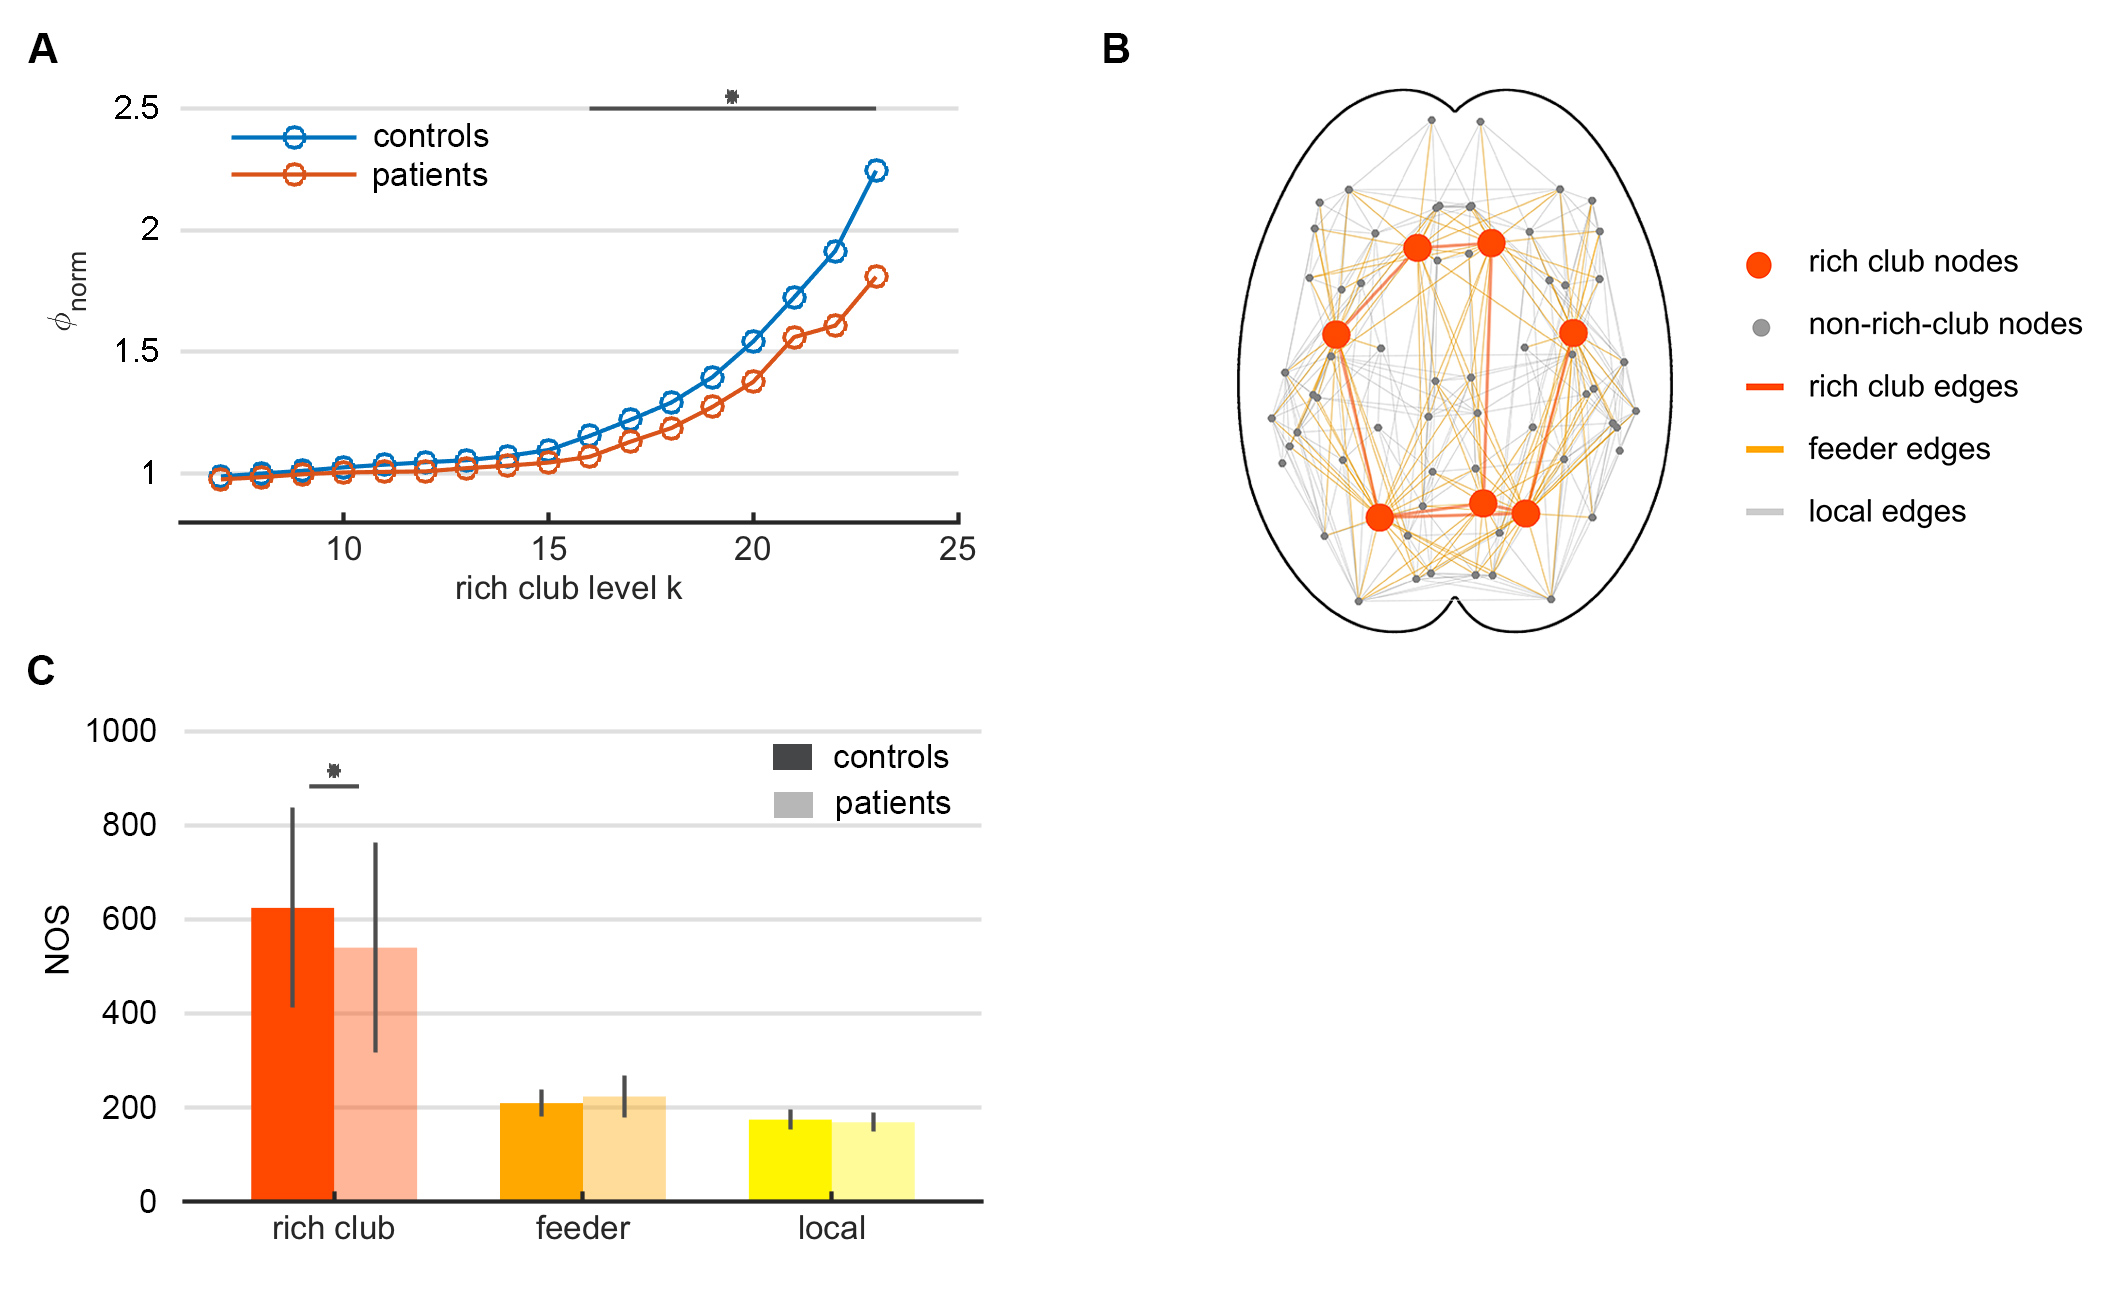
\includegraphics[width=\linewidth]{images/rcsczFig1.jpg}
  \caption{(A) Decreased rich club coefficient in patients (red) as compared with healthy controls (blue) for degree \textit{k} ranging from 16 to 23 (\pval = 0.012, 10,000 permutations, uncorrected). (B) Group-averaged structural network for healthy controls. Rich club regions (red) were identified by setting the threshold as degree > 18, including bilateral superior frontal gyri, superior parietal lobules, insula, and left precuneus. Connections were classified into 3 categories: rich club (red), feeder (orange), and local (gray) connections. (C) Group-averaged connectivity strength (number of streamlines [NOS] weighted) of the rich club (red), feeder (orange), and local (yellow) connections in healthy controls (dark) and patients (light). Error bars represent one standard deviation. Patients showed decreased rich club connection density in comparison with healthy controls (\pval = 0.032, 10,000 permutations, uncorrected).
}
  \label{rcsczFig1}
\end{figure}

\subsection*{SC-FC coupling}
Overall FC strength (average of the FC matrix) was found to be similar across patients and controls (\pval = 0.408, 10,000 permutations), as was the FC strength of rich club, feeder, and local connections (\pval > 0.526, 10,000 permutations). Both patients and healthy controls demonstrated a positive correlation between overall SC and FC values, with a mean (standard deviation) SC-FC correlation coefficient of 0.271 (0.064) for patients and 0.272 (0.060) for controls (Figure \ref{rcsczFig2}). SC-FC coupling was similar in patients compared to controls (\pval = 0.461, 10,000 permutations). Considering the distinct connection categories, a significantly reduced SC-FC coupling was detected for rich club connections in patients compared to controls (\pval < 0.001, 10,000 permutations, NOS-weighted), whereas no such difference in SC-FC coupling was found in feeder (\pval = 0.865) and local (\pval = 0.414) connections (Figure \ref{rcsczFig2}). Similar effects were found when correcting for age and gender (\pval < 0.001, 10,000 permutations) and when using SC networks weighted by SD (\pval < 0.001, 10,000 permutations).

\begin{figure}[h]
\centering
  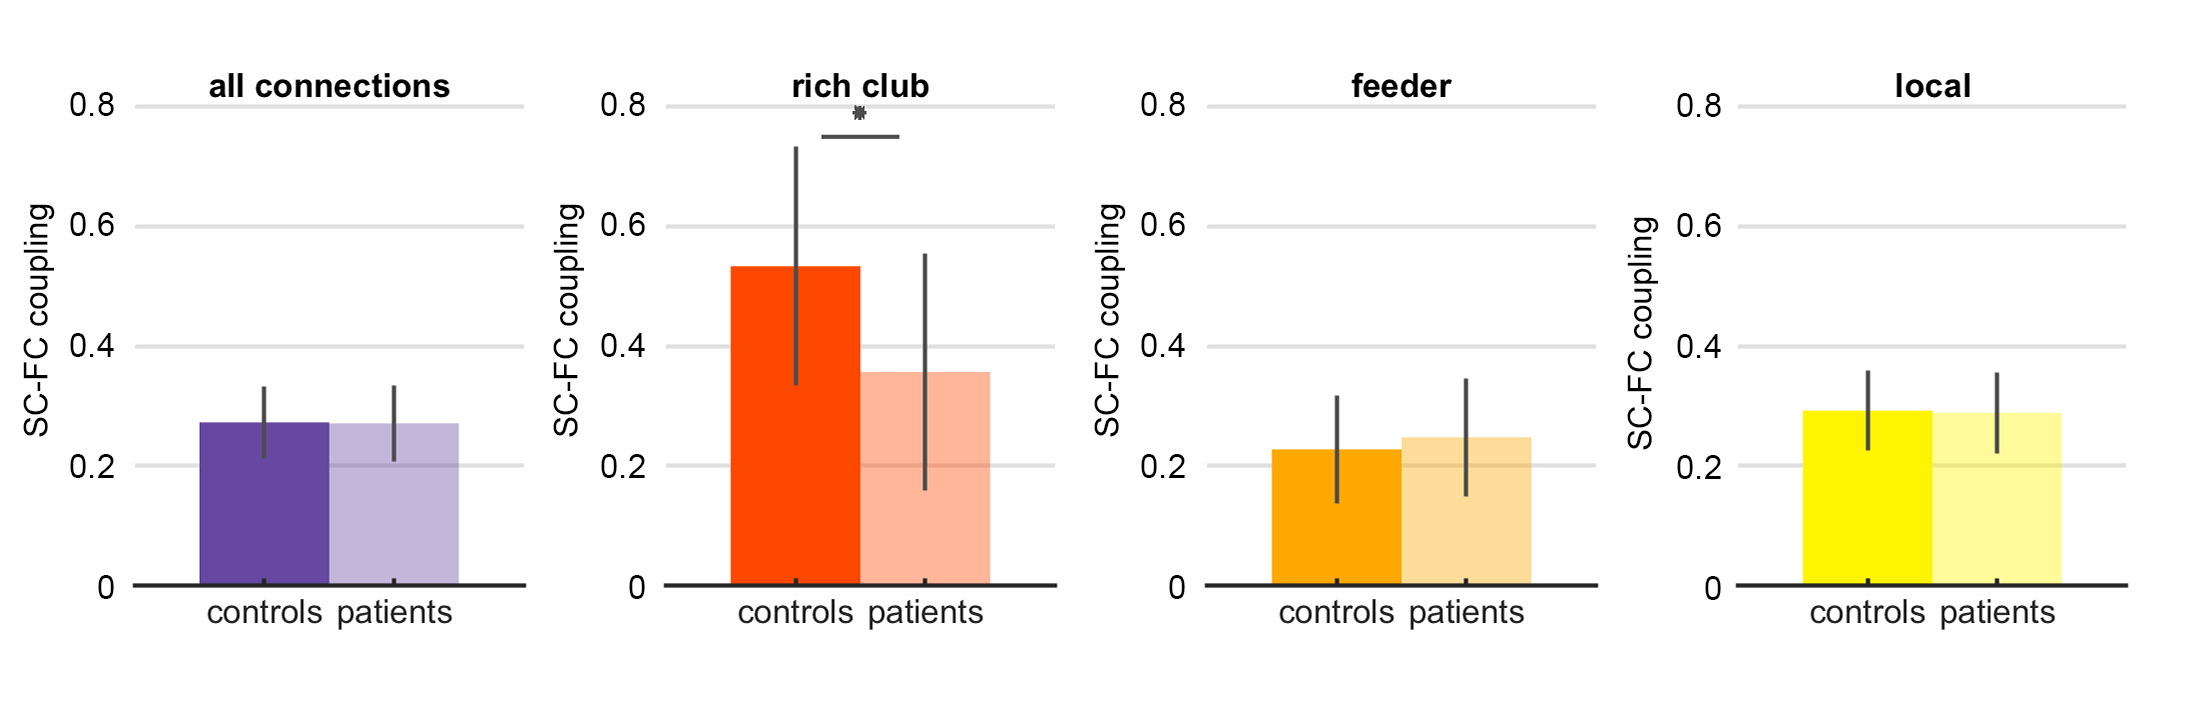
\includegraphics[width=\linewidth]{images/rcsczFig2.jpg}
  \caption{\small SC-FC coupling in healthy controls (dark) and patients (light) for all connections, rich club connections (\pval < 0.001, 10,000 permutations, false discovery ratio [FDR] corrected), feeder connections (no effect), and local connections (no effect). Error bars represent one standard deviation and asterisk indicates significance.}
  \label{rcsczFig2}
\end{figure}

\subsection*{Correlation between network organization and clinical Variables}
No specific association between rich club connections' strength and symptom scores was observed. In patients, the strength of feeder connections was found to be negatively correlated with PANSS positive score (NOS, \rval = -0.34, \pval = 0.030) and total score (\rval = -0.35, \pval = 0.022), suggesting that patients with weaker feeder connections may have more severe symptoms, especially with regard to positive symptoms. Strength of local connections was negatively correlated with PANSS positive score (NOS, \rval = -0.32, \pval = 0.043) and negative score (NOS, \rval = -0.36, \pval = 0.019) (Figure \ref{rcsczFig3}). No specific correlation was found for SD connectivity.

\begin{figure}[H]
\centering
  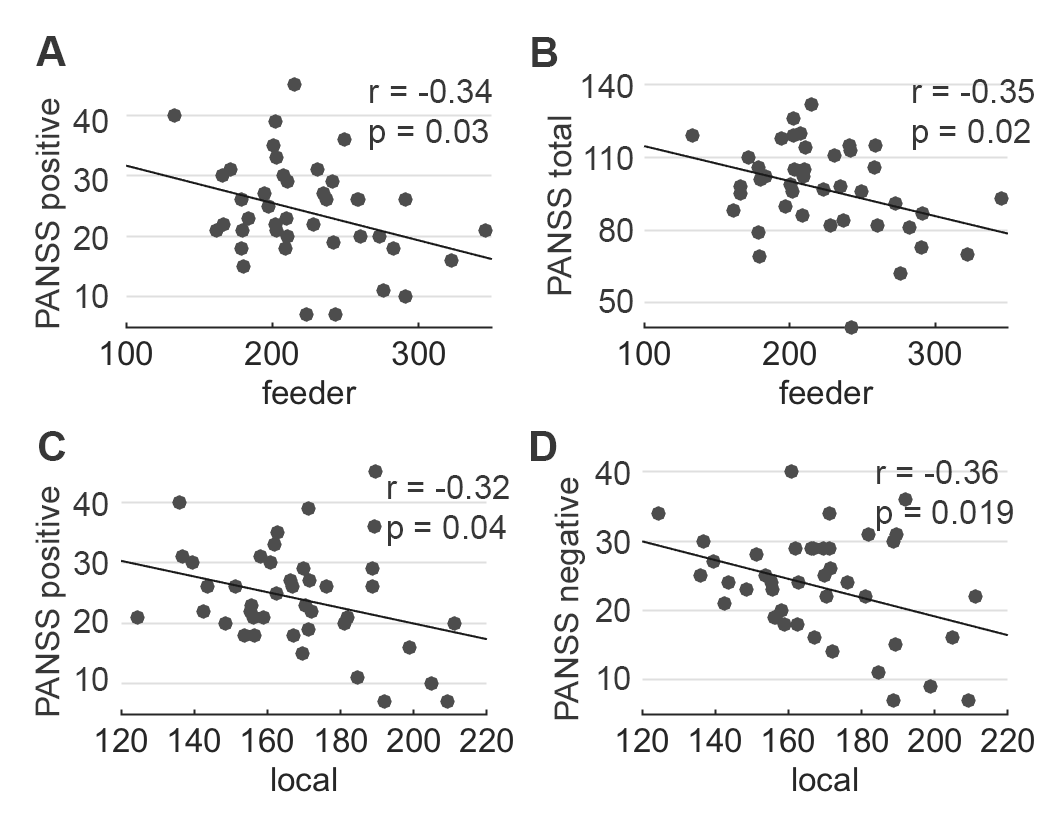
\includegraphics[width=8cm]{images/rcsczFig3.png}
  \caption{Feeder connections (NOS) were negatively correlated with (A) PANSS positive score (\rval = -0.34, \pval = 0.030, uncorrected) and (B) total score (\rval = -0.35, \pval = 0.022, uncorrected) in patients. Local connections (NOS) were negatively correlated with (C) PANSS positive score (\rval = -0.32, \pval = 0.043, uncorrected) and (D) negative score (\rval = -0.36, \pval = 0.019, uncorrected).}
  \label{rcsczFig3}
\end{figure}

\subsection*{Machine learning disease classification}
To explore the performance of classification using connectome measurements, we trained a quadratic support vector machine (SVM, see Supplementary Methods) based on structural connectivity strength and SC-FC coupling of rich club connections (see Supplementary Methods). Using five-fold cross-validation, we obtained a prediction accuracy of 73.3\% (sensitivity = 76\% and specificity = 71\%; Supplementary Figure \ref{figureS4:confusionmatrix}).

\subsection*{Replication dataset}
Patients' rich club effects were validated using the replication dataset. The cortical rich club was taken as the same set of regions as in the principal dataset (the two datasets showed high consistency in rich club organization, see supplementary results). Patients (10 medication-na\"{i}ve patients; results for the full replication dataset including 29 additional patients with a short medication history are shown in supplementary results) again showed a significant reduction in rich club connectivity strength compared with healthy controls (NOS, \pval = 0.021, 10,000 permutations), with no difference observed in feeder (\pval = 0.394) or local (\pval = 0.602) connections (Figure \ref{rcsczFig4}). Examining the SD of rich club connections showed similar results (rich club connectivity \pval = 0.015, 10,000 permutations). A marginal effect of reduced SC-FC coupling was observed for rich club connections (\pval = 0.048), with no effect for feeder (\pval = 0.713) and local (\pval = 0.921) connections.

\begin{figure}[h]
\centering
  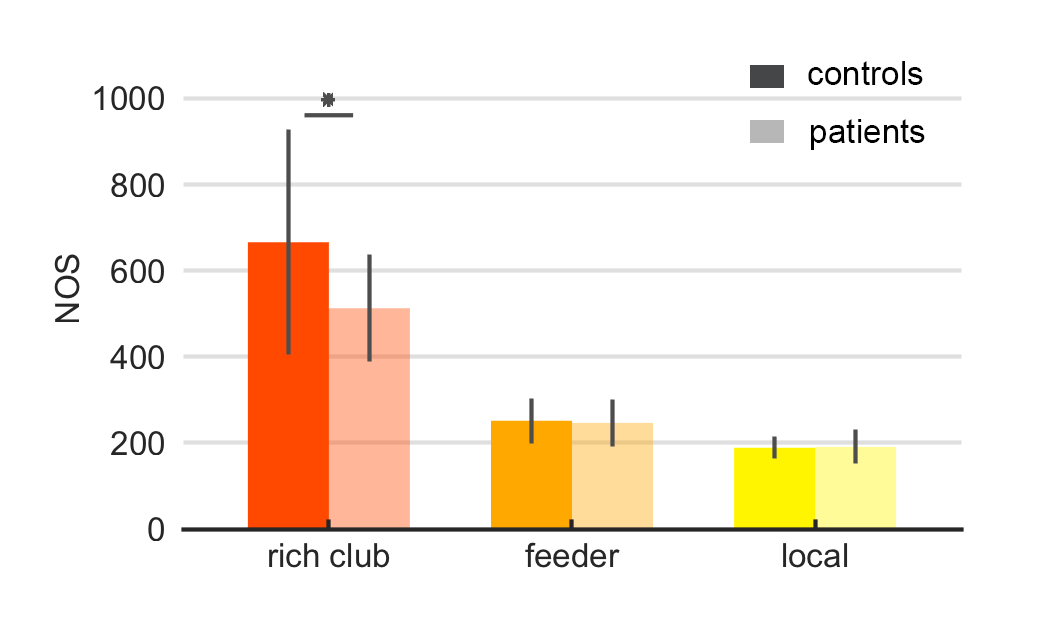
\includegraphics[width=8cm]{images/rcsczFig4.png}
  \caption{Replication dataset. Patients showed reduced rich club connection strength compared with healthy controls (NOS, \pval = 0.021, 10,000 permutations, uncorrected). No difference was observed in feeder (\pval = 0.394) and local connections (\pval = 0.602). Error bars represent one standard deviation and asterisk indicates significance.}
  \label{rcsczFig4}
\end{figure}


\section*{Discussion}
We investigated brain network organization in a sample of untreated, medication-na\"{i}ve first-episode schizophrenia patients. Rich club organization and structure-function coupling of rich club connections were found to be altered in patients compared to controls, suggesting that rich club organization may be already impaired in the early stages of schizophrenia.

Previous studies have noted the potential influence of medication on brain network findings in schizophrenia \citep{Crossley2017ConnectomicCO}. In the current study, we took extra care to rule out medical and therapeutic effects by examining first-episode, medication-na\"{i}ve patients. Our results suggest that the impairment of rich club organization directly relate to schizophrenia independently from possible confounding factors, advancing our understanding of the disease mechanisms during the early stages of the disorder.

Previous studies have reported aberrant rich club connectivity and functional brain dynamics in European chronic schizophrenia patients \citep{vanDenHeuvel2013AbnormalRC}. Similar findings have been reported in a cohort of North American chronic schizophrenia patients \citep{Yeo2016GraphMO} and, recently, in a large sample of Australian patients with schizophrenia or schizoaffective disorder \citep{Klauser2017WhiteMD}. Our study consolidates and extends these previous findings by showing an alteration of rich club organization in a cohort of Chinese patients and further underscores the cultural ubiquity of the biological underpinnings of schizophrenia.

Studies examining brain abnormalities in first-episode schizophrenia have reported fiber tract disruptions in the anterior limb of internal capsule \citep{Weiss2015ImprovedNA,Kelly2017WidespreadWM}, cingulum \citep{Xiao2018WhiteMA}, and anterior corona radiate \citep{Caprihan2015ThePR,Xi2016TheSC,Asmal2017InsightAW,Subramaniam2017WhiteMM}. The rich club regions identified in this study, i.e., the bilateral superior frontal gyri, superior parietal lobules, and insula, as well as the precuneus, are located in parts of the brain interconnected by the above-mentioned white matter tracts \citep{Greicius2008PersistentDN,vanDenHeuvel2009FunctionallyLR}. Rich club disruption is coherent with previous findings on schizophrenia patients \citep{vanDenHeuvel2013AbnormalRC,Collin2014ImpairedRC} and suggests that brain network alterations may be concentrated around the centrally connected areas of the human brain \citep{Klauser2017WhiteMD,Greicius2008PersistentDN,vanDenHeuvel2009FunctionallyLR}. In such highly connected fronto-parietal areas, myelination has been suggested to continue postnatally until the third decade of life \citep{Marn2016DevelopmentalTA,Silbereis2016TheCA}, which overlaps with the most frequent period of schizophrenia onset, occurring mostly in the early- to mid-20s for men and late-20s for women \citep{Abbas2013DIAGNOSTICAS}. Therefore, our observed structural rich club findings in first-episode patients may indirectly reflect an important neurodevelopmental feature of schizophrenia.

With converging evidence pointing to a rich club white matter impairment in both early and chronic stages of schizophrenia, a critical next step will be to determine and assess the potential value of these features in clinical applications. "Radiomics," defined as "the conversion of images to higher-dimensional data and the subsequent mining of these data for improved decision support," \citep{Gillies2016RadiomicsIA} represents the next step in promoting the translation \citep{Aerts2016ThePO} of brain connectome-based features to diagnosis and prediction for schizophrenia. A radiomics analysis involves the high-throughput extraction of meaningful measures (such as rich club connectivity) from medical images to support clinical decision processes \citep{Gillies2016RadiomicsIA}. Previous studies have suggested that gray matter abnormalities in schizophrenia are frequent, but quite heterogeneous across patients \citep{Wolfers2018MappingTH}, potentially limiting the contribution of gray matter features as a single biomarker for the disorder. Using machine learning techniques as a post-hoc analysis, we demonstrated the potential validity of individual rich club organizations (Supplementary Figure \ref{figureS3:scatter_scfc_nos}) for the classification of first-episode schizophrenia patients (see Supplementary Methods). Recent findings have shown that functional connectome organization may be an important source of information to predict the conversion to psychosis in a high-risk population \citep{Collin2018FunctionalCO}. Future studies combining multi-modal neuroimaging features may facilitate the identification of schizophrenia and further improve psychiatric care.

Several comments regarding the used methods and results need to be addressed. First, examining first-epi- sode schizophrenia patients, we obtained some distinct results compared to previous studies examining chronic schizophrenia \citep{vanDenHeuvel2013AbnormalRC,Yeo2016GraphMO,Klauser2017WhiteMD}. A decrease in SC-FC coupling was found in rich club connections in first-episode patients in our study, while an increase in SC-FC coupling in whole-brain connections has been observed in treated, chronic schizophrenia patients \citep{vanDenHeuvel2013AbnormalRC}. The heterogeneity of these findings could reflect the effects of medication and/or of the clinical history of the patients, but further investigation is warranted. Investigating the whole replication dataset (10 medication-na\"{i}ve and 29 treated patients) did not reveal alterations in rich club SC-FC coupling (\pval = 0.102 for NOS and 0.113 for SD). A second comment concerns the use of diffusion-weighted MRI and deterministic tractography to reconstruct cortico-cortical white matter pathways, as these methods are well-known to have several caveats regarding the reconstruction of complex oriented pathways \citep{Jbabdi2011TractographyWD}. We used a common clinical DWI protocol with a singleb-value of 1000 s/mm\textsuperscript{2}, which might be insufficient to resolve complex crossing fibers in the tractography \citep{Weiss2015ImprovedNA,Tournier2007RobustDO,Tournier2004DirectEO}. The use of higher magnetic field strength, higherb-value, more diffusion directions, and methods suitable for the reconstruction of complex fiber orientations (e.g., probabilistic tractography \citep{Behrens2007ProbabilisticDT} or constrained spherical deconvolution \citep{Tournier2007RobustDO,Tournier2004DirectEO}) may result in better reconstruction of white matter fiber pathways. Third, head movements during fMRI acquisition have been argued to be an important source of spurious signals in functional connectivity studies \citep{Power2012SpuriousBS,Yan2013ACA}. In this study, we performed scrubbing to reduce the effect of head motion, and including the head movement measures and number of scrubbed frames as covariates to the group-comparison statistical analyses revealed consistent findings (see supplementary results). Fourth, brain network architecture was characterized by means of graph theoretical metrics that have received large consensus in clinical connectome literature \citep{Fornito2012SchizophreniaNA,Heuvel2014BrainNI,Griffa2013StructuralCI,Fornito2015ConnectomicsAN}. Nevertheless, it has been noted that graph metrics can be highly correlated in real-world networks \citep{sporns_human_2005} and new network measures are continuously proposed \citep{Bertolero2017TheDC,Betzel2017MultiscaleBN}. Future research applying advanced network measures could bring further insights into the characteristics of brain network alterations in early schizophrenia and the clinical diagnosis.

This study shows a reduced level of structural rich club connectivity in first-episode schizophrenia patients with no or limited medication history. We suggest that connectome features including rich club impairment reflect pathophysiological processes occurring early in the course of schizophrenia, independently from the medication history of the patients. Our results are important for advancing our understanding of the neuropathological mechanisms of first-episode schizophrenia. They add important empirical support for the use of individual connectome organization as a potential marker for disease classification.
    
\section*{Funding}
This work was supported by the National Natural Science Foundation of China (grants 81801675 to L.-B.C., 81571651 to H.Y.); the State Scholarship Fund, China Scholarship Council (grants 201506040039 to Y.W., 201603170143 to L.-B.C); the Netherlands Organization for Scientific Research (grants ALWOP.179 and VIDI- 452-16-015 to M.P.vdH.); a fellowship of MQ (to M.P.vdH.); and the Swiss National Science Foundation (grant \#P2ELP3\_172087 to A.G.).

\section*{Acknowledgments}
We would like to acknowledge, with special thanks, Miss Xiao Chang at Department of Psychiatry, Brain Center Rudolf Magnus, University Medical Center Utrecht and Prof. Qingrong Tan and Prof. Huaning Wang at Department of Psychiatry, Xijing Hospital, Fourth Military Medical University for their help on this work.

\printbibliography[heading=subbibliography]

\end{refsection}

% SI
\begin{refsection}
\newpage
\section*{Supplementary Information}
\subsection*{Supplementary Methods}
\subsubsection*{Participants}
All subjects were right handed and their biological parents were of the Han Chinese ethnic group. Exclusion criteria for patients included: (1) presence of another psychiatric disorder; (2) history of receiving antipsychotics (or more than two weeks of antipsychotic medication for the replication dataset), history of repetitive transcranial magnetic or current stimulation, or a history of behavioral treatment; (3) history of clinically significant neurological, neurosurgical or medical illnesses; (4) substance abuse within the prior 30 days or substance dependence within the prior 6 months; (5) pregnancy or any other MR imaging contraindications, e.g., cardiac pacemakers and other metallic implants. Exclusion criteria for healthy controls included: (1) presence of any psychotic syndrome; (2) history of receiving antipsychotics, repetitive transcranial magnetic stimulation, transcranial current stimulation, or behavioral treatment; (3) history of clinically significant neurological, neurosurgical or medical illnesses; (4) substance abuse within the prior 30 days or substance dependence within the prior 6 months; (5) pregnancy or MR imaging contraindications, e.g., cardiac pacemakers and other metallic implants. In total, out a selected group of 113 patients and 124 controls, thirty-two patients and ten controls were excluded because of image quality and high head motion, resulting in the examined population of 81 patients and 114 controls. Dose of current antipsychotic drugs at time of MRI was converted using defined daily dose method (WHO Collaborating Centre for Drug Statistics Methodology, 2014) \citep{Leucht2016DoseEF}.

\subsubsection*{Data preprocessing}
\textit{T1-weighted images.} Cortical parcellation was obtained on the basis of T1-weighted images using the Freesurfer software (version 5.3.0). The automated recon-all pipeline was used, including segmentation of gray and white matter tissue, reconstruction of cortical mantle, and parcellation of the cortical mantle into 68 cortical areas. Cortical segmentations were checked manually for accuracy. 68 cortical regions (34 per hemisphere) were segmented according to the Desikan Killiany atlas \citep{DESIKAN2006968}. Two further subdivisions \citep{CAMMOUN2012386} (114 regions, 57 per hemisphere; and 219 regions, 108 in the right hemisphere and 111 in the left hemisphere) of the Desikan Killiany atlas were additionally used for validation purposes.

\textit{Diffusion weighted imaging (DWI).} Sixty-four DWI images (single-shell, b = 1000 s/mm$^{2}$) and a b = 0 image were realigned and corrected for small head movements and common gradient-induced distortions \citep{ANDERSSON2002177}. The diffusion profile within each voxel was reconstructed using generalized q-sampling imaging (GQI) \citep{YEH2010}. In addition, fractional anisotropy (FA) maps were computed from fitted single tensors \citep{Chang2005RESTORERE}. Deterministic tractography was performed to reconstruct white matter tracts, applying the Fiber Assignment by Continuous Tracking (FACT) algorithm \citep{Mori2002FiberTP}. For each white matter voxel, eight streamline seeds were started and tracking was stopped if the streamline reached a voxel of low fractional anisotropy (FA < 0.1), exited the gray matter/white matter mask, or made a sharp turn (> 45$^{\circ}$). All preprocessing steps were performed according to previous studies \citep{VANDENHEUVEL2016293,Romme2017ConnectomeDA}.

\textit{Resting-state functional magnetic resonance imaging (rs-fMRI).} Resting-state fMRI data of each subject were realigned and co-registered with the T1-weighted image to overlap with the resultant cortical parcellation maps. Second, the blood oxygenation level-dependent (BOLD) time series were corrected for linear trends, as well as global nuisance covariance, including 6 head motion parameters and mean signals of white matter and ventricles. Third, band-pass filtering (0.01-0.1 Hz) was performed together with motion scrubbing to minimize the influence of head-motion \citep{Power2012SpuriousBS}. Each slice with framewise displacement (FD) exceeding 0.25 (defined as the sum of the absolute derivatives of the six realignment parameters) and dynamic variability (DVARS) exceeding 1.5, as well as 1 back neighbour, were removed following the procedure by Power et al. \citep{Power2012SpuriousBS}.

\subsubsection*{Graph metrics}
\textit{Connectivity strength.} Connectivity strength (\textit{S}) was computed as the average weight of all connections within the network as follows:
\[\mathsf{S=\overline{W}}\]
where \textit{W} indicates connectivity weights of the reconstructed network edges.\\

\noindent
\textit{Network density.} Network density (\textit{D}) was computed by dividing the number of connections existed in the network by the number of connections in the fully-connected network as follows:
\[\mathsf{D=\frac{E}{n(n-1)/2}}\]
with \textit{E}, the number of connections and \textit{n}, the number of nodes.\\

\noindent
\textit{Clustering coefficient.} Clustering coefficient, \textit{Ci}, reflects the level of local connectedness of a node, and was computed by dividing the geometric mean of triangles around a node by the maximum number of possible triangle around a node. The global level of clustering coefficient was obtained by averaging the clustering coefficient of all nodes within the network as follows:
\[\mathsf{C=\frac{1}{n}\sum_{i \in N} \frac{\sum_{j,h \in N} (w_{ij}w_{ih}w_{jh})^{1/3}}{k_{i}(k_{i}-1)}}\]
where \textit{N} the set of all nodes and $\mathsf{k_{i}}$ the degree of node \textit{i} (i.e., the number of connections linked to node \textit{i}). Normalized clustering coefficient \textgamma, was obtained by comparing the clustering coefficient in brain network to those in 1000 random networks as follows:
\[\mathsf{\gamma=\frac{C}{\overline{C_{random}}}} \]   \\

\noindent
\textit{Shortest path length.} The shortest path (\textit{d}) between two nodes was taken as the minimum edges' weights needed to traverse from one node to the other \citep{RUBINOV20101059}. The mean shortest path length of a network (\textit{L}) was taken as the average shortest path length between all pairs of nodes in the network as follows:
\[\mathsf{L=\frac{1}{n} \sum_{i \in N} {\frac{\sum_{j \in N,j \neq i} {d_{ij}}}{n-1}}}\]
Normalized path length \textlambda \ was computed by dividing the mean shortest path length in brain network by those in 1000 random networks as follows:
\[\mathsf{\lambda=\frac{L}{\overline{L_{random}}} }\] \\

\noindent
\textit{Rich club.} Weighted rich club coefficient $\mathsf{\Phi_{w}(k)}$ was assessed \citep{Opsahl2008ProminenceAC}. First, all connections of the network (weighted by streamline count) were ranked according to their weight, resulting in a vector $\mathsf{W^{ranked}}$. Second, sub-networks containing nodes with a degree larger than \textit{k} (where degree is the number of binary connections linked to each node) were selected for \textit{k} ranging from 5 to 40. Third, the number of edges within the selected sub-network ($\mathsf{E_{>k}}$) was determined and the sum of their weights ($\mathsf{W_{>k}}$) was computed. Fourth, the strongest $\mathsf{E_{>k}}$ edges of the whole network were selected and summed up, as computed by summing the top $\mathsf{E_{>k}}$ edges' weights in the ranked weights $\mathsf{W^{ranked}}$. Finally, the weighted rich club parameter $\mathsf{\Phi_{w}(k)}$ was computed as the ratio between $\mathsf{W_{>k}}$ and the sum of the strongest number of links $\mathsf{E_{>k}}$ in the total network by the following:
\[\mathsf{\Phi^{w}(k)=\frac{W_(>k)}{\sum_{l=1}^{E_{>k}} w^{ranked}_{l}}}\]
The weighted rich club parameter $\mathsf{\Phi_{w}(k)}$ was normalized by comparing to 1,000 random networks, to determine to what extent the observed connection strength between rich club nodes exceeds that predicted by the random null model, driven by node degree alone. Normalized rich club coefficient $\mathsf{\Phi_{norm}(k)}$ was computed as the ratio of $\mathsf{\Phi_{w}(k)}$ in the brain network to the mean of $\mathsf{\Phi_{random}(k)}$ across random networks, 
\[\mathsf{\Phi_{norm}(k)=\frac{\Phi(k)}{\Phi_{random}(k)} }\]
with a normalized rich club coefficient $\mathsf{\Phi_{norm}(k)}$ > 1 expressing the presence of a rich club organization in the network. Random networks were generated by shuffling edges in the structural network, preserving connection weights and the (binary) degree distribution \citep{Maslov2002SpecificityAS}. The rich club coefficient was computed until less than three nodes could be included in the examined set. Graph metrics and null models were computed using the MATLAB-based Brain Connectivity Toolbox \citep{RUBINOV20101059}.

\subsubsection*{Rich club nodes}
Rich club nodes were defined by selecting the nodes with degree \textit{k} \ > 18 in the group-averaged structural network of all subjects, resulting in 7 hub nodes (top 10\% percent high degree nodes in the network). Alternatively, we selected rich club nodes on the basis of individual structural networks of all subjects by setting the rich club threshold as degree > 18 and choosing the top 10\% mostly consistent rich nodes across subjects. A similar set of nodes was identified, including bilateral superior parietal lobe, superior frontal lobe, precuneus, and right insula. Furthermore, we also used a range of degree levels (\textit{k} \ > 14 - 22) as thresholds to define rich club nodes and observed similar findings (Supplementary Results). Results were thus consistent across different types of rich club selection.

\subsubsection*{Machine learning classification analysis}
Taking the principle dataset, a machine learning quadratic support vector machine (SVM) was fitted to the data of connectivity weights (NOS) and SC-FC coupling of rich club connections, as well as other demographic features, such as age, gender, and education time. Validation analysis was performed using 5-fold cross-validation (i.e., data samples were divided into 5 sub-datasets, with 4 sub-datasets taken as the training datasets and the other as the validation dataset, iterating for 5 times). Accuracy was calculated for the fitted model as the proportion of true predictions among the total number of cases. Sensitivity and specificity were computed as the proportions of actual positives and actual negatives that were correctly identified, respectively. Training was performed using the Classification Learner App embedded in MATLAB R2018a.

\subsection*{Supplementary Results}
\subsubsection*{Validation dataset}
\textit{Graph metrics.} The replication dataset used in the main text (i.e., only 10 untreated patients included) demonstrated no group difference for the network density (\pval = 0.428), connectivity strength (\pval = 0.622), clustering coefficient (\pval = 0.992), normalized clustering \textgamma, \pval = 0.819), and shortest path length (\pval = 0.135). Patients showed a slight increase in normalized shortest path length \textlambda \ compared to controls (\pval = 0.019).\\

\noindent
\textit{Using the whole dataset.} Here we reported results obtained by including 39 first-episode schizophrenia patients (10 untreated, medication na\"{i}ve patients and 29 patients with no more than two weeks of cumulative exposure to antipsychotics). Similar as in the discovery principal dataset, no difference was observed for network density (\pval = 0.171), connectivity strength (\pval = 0.073), and clustering coefficient (\pval = 0.554; for normalized \textgamma, \pval = 0.491). A slight reduction in shortest path length (\pval = 0.018; for normalized \textlambda, \pval = 0.008) in patients as compared to controls was observed.

With respect to the rich club structure, patients showed a significant reduction in rich club connection strength compared with healthy controls (NOS, \pval = 0.025, 10,000 permutations), with no difference observed in feeder (\pval = 0.117) and local connections (\pval = 0.137). Examining the streamline density of rich club connections showed a non-significant attenuated effect (\pval = 0.083, 10,000 permutations). Considering the slight age bias in replication dataset (\pval = 0.086), we excluded the six oldest subjects from control group (\pval = 0.403 after exclusion) to examine the potential effect of age on our results. Analyses on the remaining subjects showed significant rich club connection disruptions in patients for the predefined rich club regions (\pval = 0.026, NOS weights). No difference of SC-FC coupling was observed in patients for rich club (\pval = 0.247), feeder (\pval = 0.808), local (\pval = 0.800) and overall (\pval = 0.807) connections. Significant SC-FC coupling reductions was observed for rich club connections with intermediate-to-long fiber distances (> 50 mm, \pval = 0.028). \\

\noindent
\textit{Rich club regions in the replication dataset.} Rich club regions selected in the principal dataset belonged to the top 11 highest degree regions observed in the replication dataset, indicating high consistency in rich club organization across the two datasets. To further verify our findings, we examined rich club nodes based on the replication dataset by choosing nodes with degree > 20 (10 nodes) in the group structural network. The selected rich club nodes included bilateral precuneus, insula, rostral middle frontal cortex, superior frontal cortex and superior parietal cortex. The effect of disruptions in the rich club connection in patients was significant (\pval = 0.035, NOS weights). SC-FC coupling for rich club, feeder, and local connections did not show differences in patients as compared to controls (\pval = 0.549, 0.960, and 0.537, separately)

\subsubsection{Comparison between schizophrenia patients from the two datasets}
To verify that patients from both cohorts were neurobiologically similar, we additionally compared the rich club organization between the two untreated first-episode schizophrenia groups used in the main results. We found that the mean NOS within the entire brain only showed a trend-level difference between the two groups of patients (\pval = 0.051, 10,000 permutations). Specifically, no difference was observed for the rich club (\pval = 0.752, 10,000 permutations) and feeder (\pval = 0.164, 10,000 permutations) connections, with only significant difference for the local connections (\pval = 0.016, 10,000 permutations). Moreover, no difference was found for the SC-FC coupling of the rich club (\pval = 0.098, 10,000 permutations), feeder (\pval = 0.239, 10,000 permutations), and local (\pval = 0.259, 10,000 permutations) connections. These findings indicated that rich club organization and functional dynamics of patients from the two cohorts were similar.

\subsubsection*{Validation of brain parcellations}
Considering the influence of different node definitions on graph properties \citep{Fornito2010NetworkSE}, findings were verified by using two finer subdivisions of the Desikan-Killiany atlas [114 regions (DK-114) and 219 regions (DK-219)] \citep{CAMMOUN2012386}. 14 out of 114 regions (12.8\%) and 21 out of 219 regions (9.6\%) were taken as rich club regions, separately. For both atlases (Supplementary Figure \ref{figureS1:dk114and250}), patients consistently showed reduced streamline volume density of rich club connections (DK-114: \pval = 0.035 and DK-219: \pval < 0.001, 10,000 permutations) in contrast to controls, while no difference was found for feeder and local connections (DK-114: \pval = 0.343 and 0.561, for feeder and local connections; DK-219: \pval = 0.261 and 0.886, for feeder and local connections, 10,000 permutations; Supplementary Figure \ref{figureS1:dk114and250}). The SC-FC coupling for rich club connections was decreased in patients (\pval = 0.008 and 0.003, separately for the two parcellations, 10,000 permutations) (Supplementary Figure \ref{figureS1:dk114and250}). Local connection weights showed negative correlation with the PANSS negative scores (\rval = -0.33 and -0.32, \pval = 0.030 and 0.054, separately) and PANSS total scores (\rval = -0.35 and -0.37, \pval = 0.021 and 0.016, separately). These findings suggest that the definition of nodes and the network size didn't affect the reported rich club changes in first-episode patients.

\subsubsection*{Validation of fiber reconstruction strategy}
In the main analysis, GQI \citep{YEH2010} was used to reconstruct the diffusion signal of voxels within the DWI data. Alternatively, we fitted the diffusion profile of each voxel to a simple tensor using a robust tensor fit method based on an M-estimator \citep{Chang2005RESTORERE} and examined our main results. Both patients and controls consistently showed a rich club structure, with a significantly decreased rich club coefficient in patients as compared with controls (\pval = 0.040, for rich club of k ranging from 16 to 23, 10,000 permutations). Furthermore, we observed a significant decrease in rich club connections (\pval = 0.047, NOS weights, and \pval = 0.023, SD weights, 10,000 permutations) and rich club SC-FC couplings (\pval = 0.001, NOS weights, and \pval = 0.003, SD weights, 10,000 permutations) in patients. Correlation analysis showed that rich club connection weights were positively correlated to the PANSS supplementary score (P4, P7, G6, S1, S2, and S3) (\rval = 0.31, \pval = 0.047). Feeder connection weights were negatively correlated to PANSS positive score (\rval = -0.35, \pval = 0.022) and total score (\pval = -0.34, \pval = 0.027). Local connection weights were also negatively correlated to PANSS negative score (\rval = -0.41, \pval = 0.006) and total score (\pval = -0.28, \pval = 0.031).

\subsubsection*{Validation of global signal correction in resting-state fMRI data}
We also evaluated the structural connectivity-functional connectivity (SC-FC) coupling alterations in patients after correcting the global signal during fMRI data preprocessing \citep{Murphy2017TowardsAC}. Patients reliably showed decreased SC-FC coupling level for rich club connections (\pval = 0.001, 10,000 permutations) compared with controls in the principle dataset, suggesting that global signal correction did not change the nature of the reported results.

\subsubsection*{FA weights}
Connections were also weighted by FA to reflect microstructure properties of white matter \citep{Beaulieu2002TheBO}. The FA-weighted structural networks in patients showed no difference in connection strength (\pval = 0.234), clustering coefficient (\pval = 0.852) or mean shortest path length (\pval = 0.344), and normalized shortest path length (\pval = 0.664). A decreased normalized clustering coefficient was observed in patients (\pval = 0.023, not corrected). The rich club coefficient showed no significant difference between the two groups (\pval > 0.112). Connection weights (i.e., mean FA) and SC-FC coupling for all three categories of connections also showed no difference between groups (\pval = 0.600, 0.887, and 0.836, for weights of rich club, feeder, and local connections, respectively; \pval = 0.766, 0.831, and 0.379, for SC-FC coupling of rich club, feeder, and local connections, respectively; 10,000 permutations).

\subsubsection*{Validation of rich club levels}
Rich club regions in the main analysis were selected by setting a rich club level of k > 18 (top 10\% high degree nodes) in the group-averaged structural network. We also performed our main analysis on the basis of a range of rich club level k from 14 (top 28\% high degree nodes) to 22 (top 3\% high degree nodes). For each k level, the average rich club connection weights (SD-weighted) are illustrated in (Supplementary Figure \ref{figureS2:range}). Rich club connection density was significantly reduced in patients as compared with controls in the range of k from 18 to 22 (\pval  < 0.05, 10,000 permutations), corresponding to 13\% to 3\% highest degree nodes included into the rich club. SC-FC coupling of rich club connections was significantly reduced in patients compared with controls in the range of \textit{k} from 14 to 20 (\pval < 0.05, 10,000 permutations) (Supplementary Figure \ref{figureS2:range}).

\subsubsection{Assessment of head motion in resting-state fMRI data}
We assessed the potential effect of head movements in the fMRI datasets. Comparing the mean FD between patients and controls showed no significant difference in both the principle dataset (\pval = 0.303) and the replication dataset (\pval = 0.103; 10,000 permutations). In the principle dataset, patients showed a larger number of scrubbed volumes compared to the controls (\pval = 0.042), but this effect was not observed in replication dataset (\pval = 0.409, 10,000 permutations). Furthermore, examining the SC-FC coupling differences between patients and controls with the mean FD and number of scrubbed volumes included as covariates showed similar results as reported in the main analysis (rich club connections: \pval < 0.001 in principle dataset and \pval = 0.024 in replication dataset; 10,000 permutations), suggestive of our results not to be driven by the effects of head motion.

\subsection*{Supplementary References}
\printbibliography[heading=none]

\newpage
\subsection*{Supplementary Tables}

\scriptsize
\captionof{table}{Detailed Scanning Parameters} \label{tableS1:MRI} 
\resizebox{\textwidth}{!}{\begin{tabular}{@{}llllclllclll@{}}\toprule
& \multicolumn{3}{c}{Siemens scanner} & \phantom{abc}& \multicolumn{3}{c}{GE scanner} \\
\cmidrule{2-4} \cmidrule{6-8}
& T1 & DWI & fMRI && T1 & DWI & fMRI \\
\midrule
TR (ms) & 2530 & 2000 & 7000 && 8.2 & 2000 & 10000 \\
TE (ms) & 3.5 & 30 & 91 && 3.2 & 30 & 82.4 \\
Flip angle ($^{\circ}$) & 7 & 90 & NA && 12 & 90 & NA \\
FOV (mm\textsuperscript{2}) & 256 × 256 & 220 × 220 & 256 × 256 && 256 × 256 & 240 × 240 & 240 × 240 \\
Matrix & 256 × 256 & 64 × 64 & 128 × 128 && 256 × 256 & 64 × 64 & 128 × 128 \\
Slice thickness (mm) & 1 & 4 & 3 && 1 & 3.5 & 2 \\
Section gap (mm) & 0 & 0.6 & 0 && 0 & 0 & 0 \\
Number of slices & 192 & 33 & 50 && 196 & 45 & 70 \\
\bottomrule
\end{tabular}}
\bigskip
\scriptsize Abbreviations: FOV, field of view; NA, not applicable; TE, echo time; TR, repetition time (ms).

\bigskip

\scriptsize
\centering
\captionof{table}{Correlations between the number of streamlines (NOS) and PANSS scores}
\label{tableS2:Corr} 
\begin{tabular}{llllll}\toprule
 &Positive&Negative&General&Supplementary&Total\\
 \midrule
NOSrc&-0.059&0.280&0.103&0.194&0.138\\
NOSfeeder&-0.335*&-0.243&-0.213&-0.023&-0.353*\\
NOSlocal&-0.316*&-0.362*&-0.016&-0.064&-0.297\\
\bottomrule
\scriptsize *  \textit{p} < 0.05, uncorrected
\end{tabular}

\bigskip

\newpage
\begin{flushleft}
\subsection*{Supplementary Figures}
\end{flushleft}

\begin{figure}[H]
\centering
  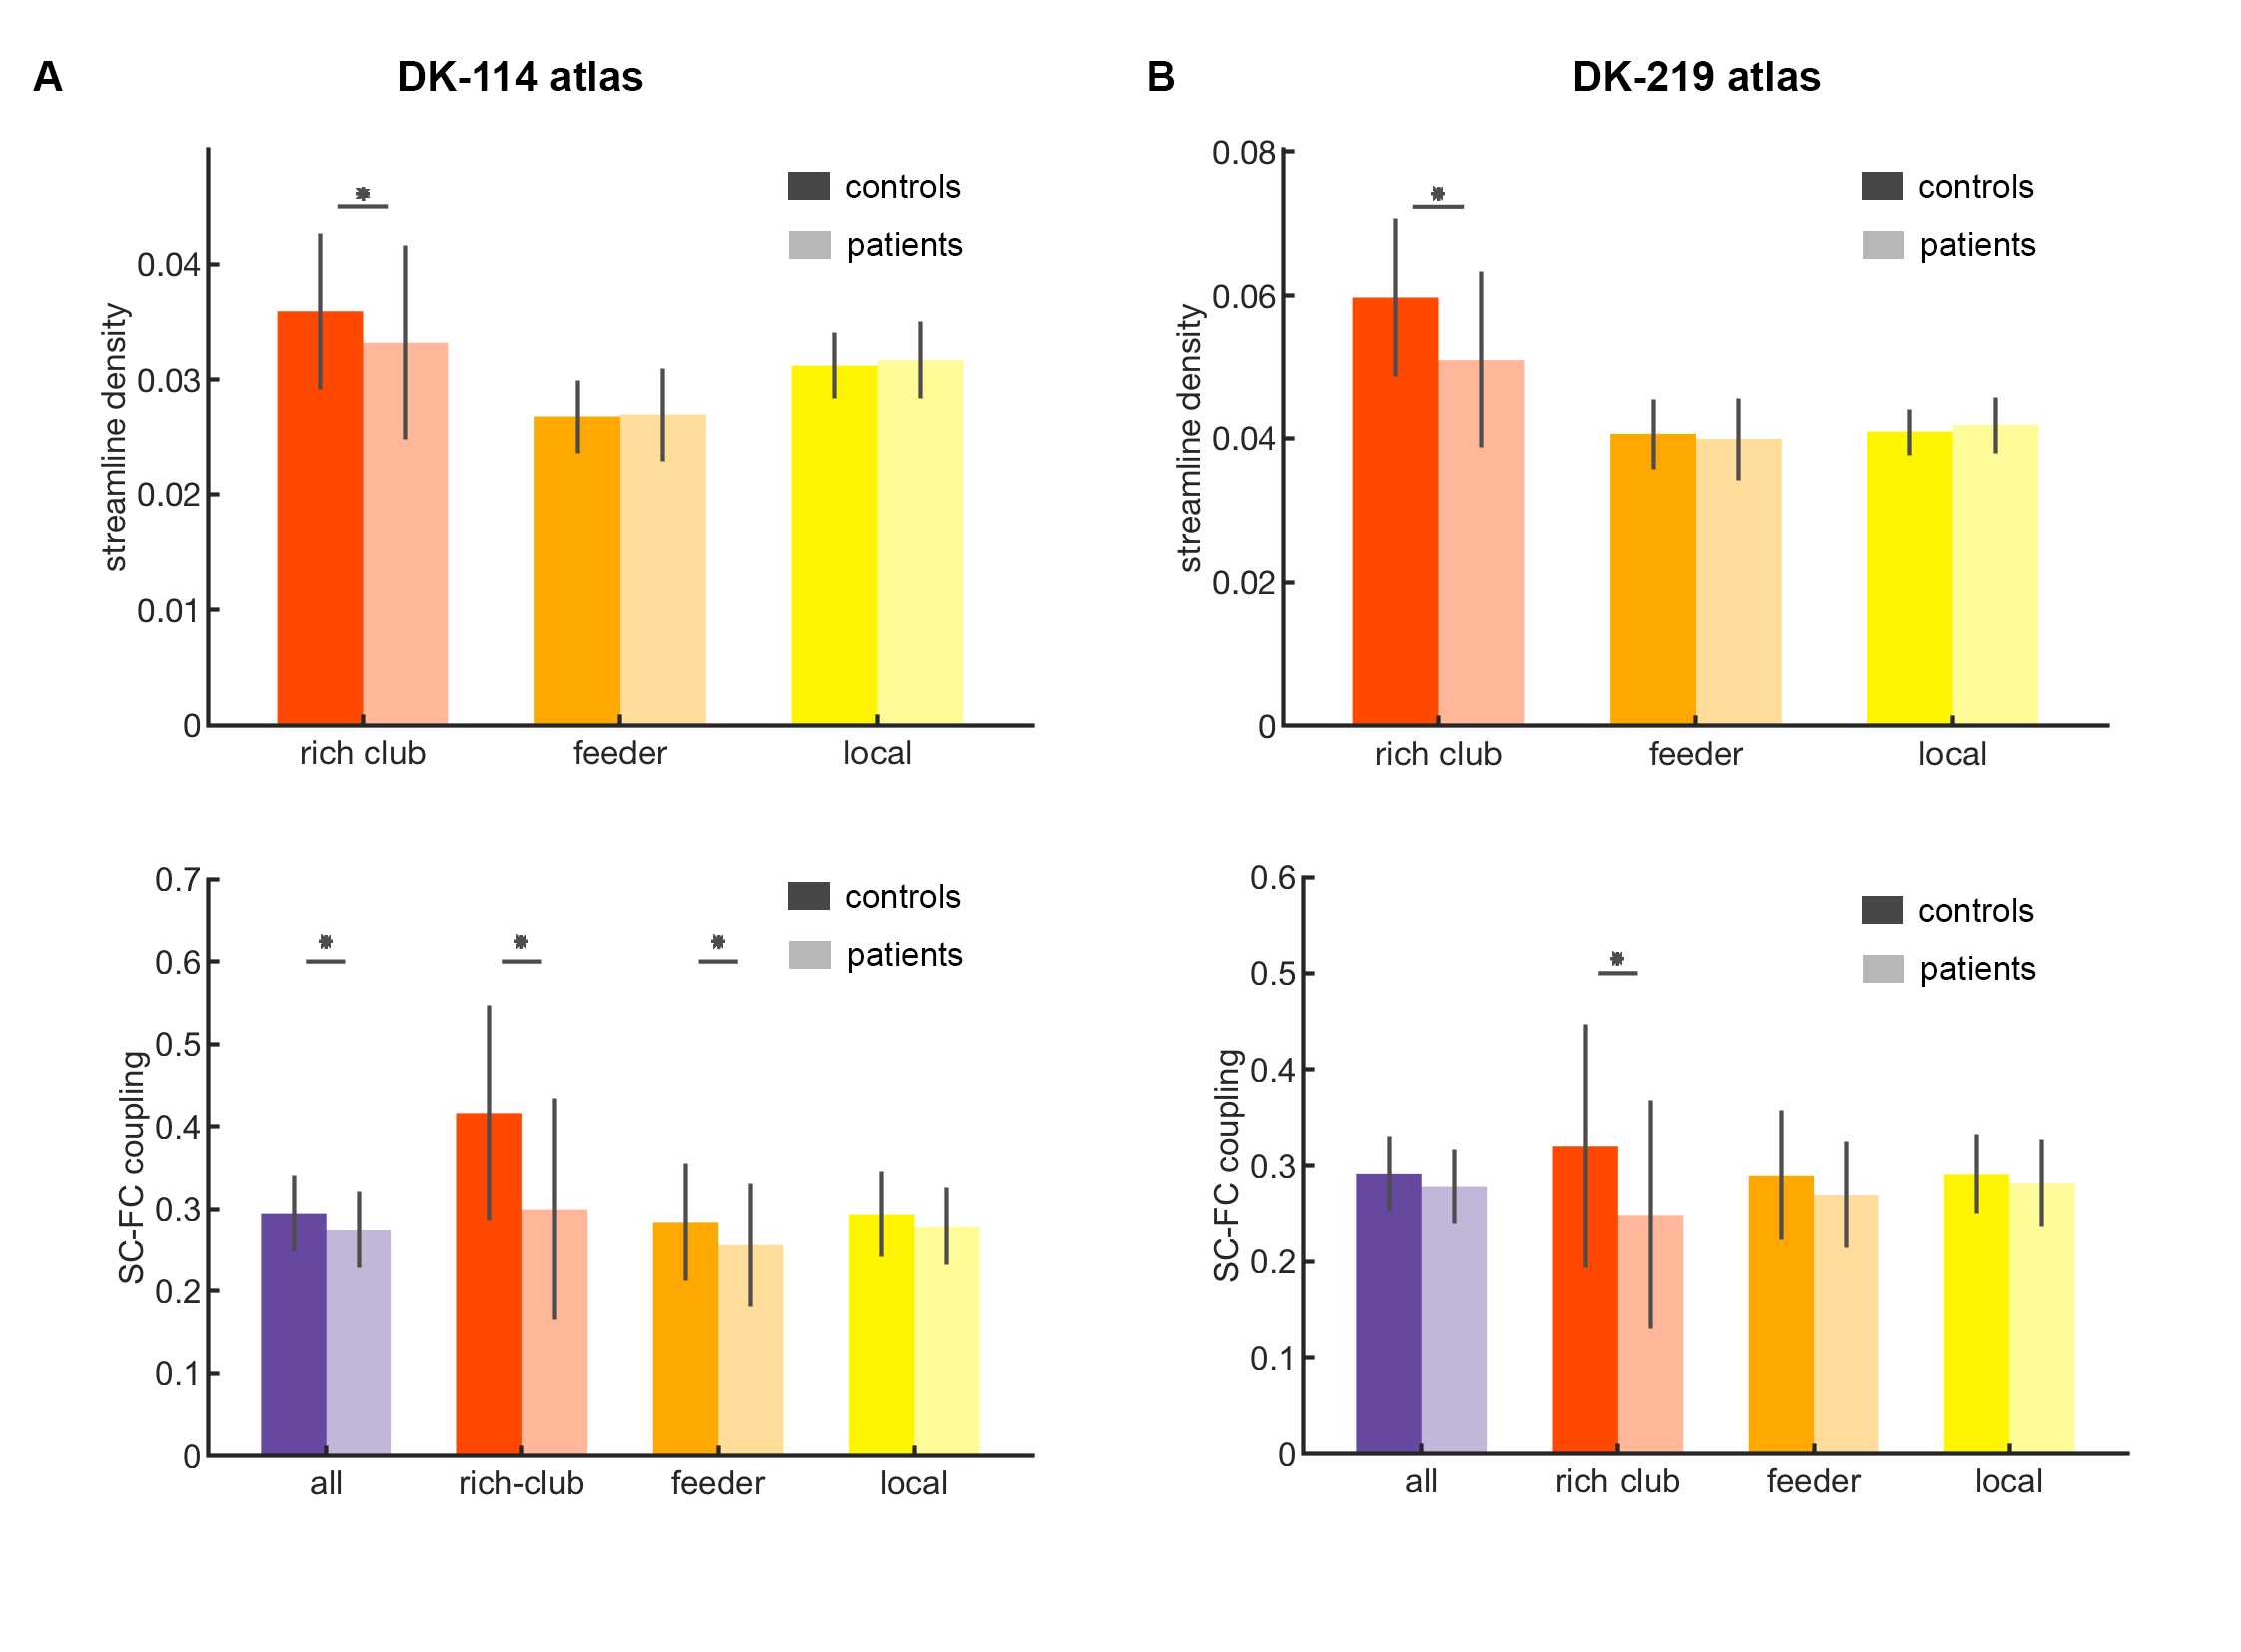
\includegraphics[width=\linewidth]{images/rcsczFigS1.png}
  \caption{\small Results using two finer subdivisions of Desikan-Killiany atlas. (A) DK-114 atlas. Top: patients showed reduced streamline volume density of rich club connections (\pval = 0.035), but not for feeder (\pval = 0.343) and local connections (\pval = 0.561). Bottom: patients showed reduced SC-FC coupling of overall (\pval = 0.023), rich club (\pval < 0.001), and feeder connections (\pval = 0.034), but not for local connections (\pval = 0.087). (B) DK-219 atlas. Top: patients showed reduced streamline volume density of rich club connections (\pval < 0.001), but not for feeder (\pval = 0.261) and local connections (\pval = 0.886). Bottom: patients showed reduced SC-FC coupling of rich club connections(\pval = 0.003), but not for overall (\pval = 0.060), feeder connections (\pval = 0.064), and local connections (\pval = 0.150).).
}
  \label{figureS1:dk114and250}
\end{figure}

\begin{figure}[H]
\centering
  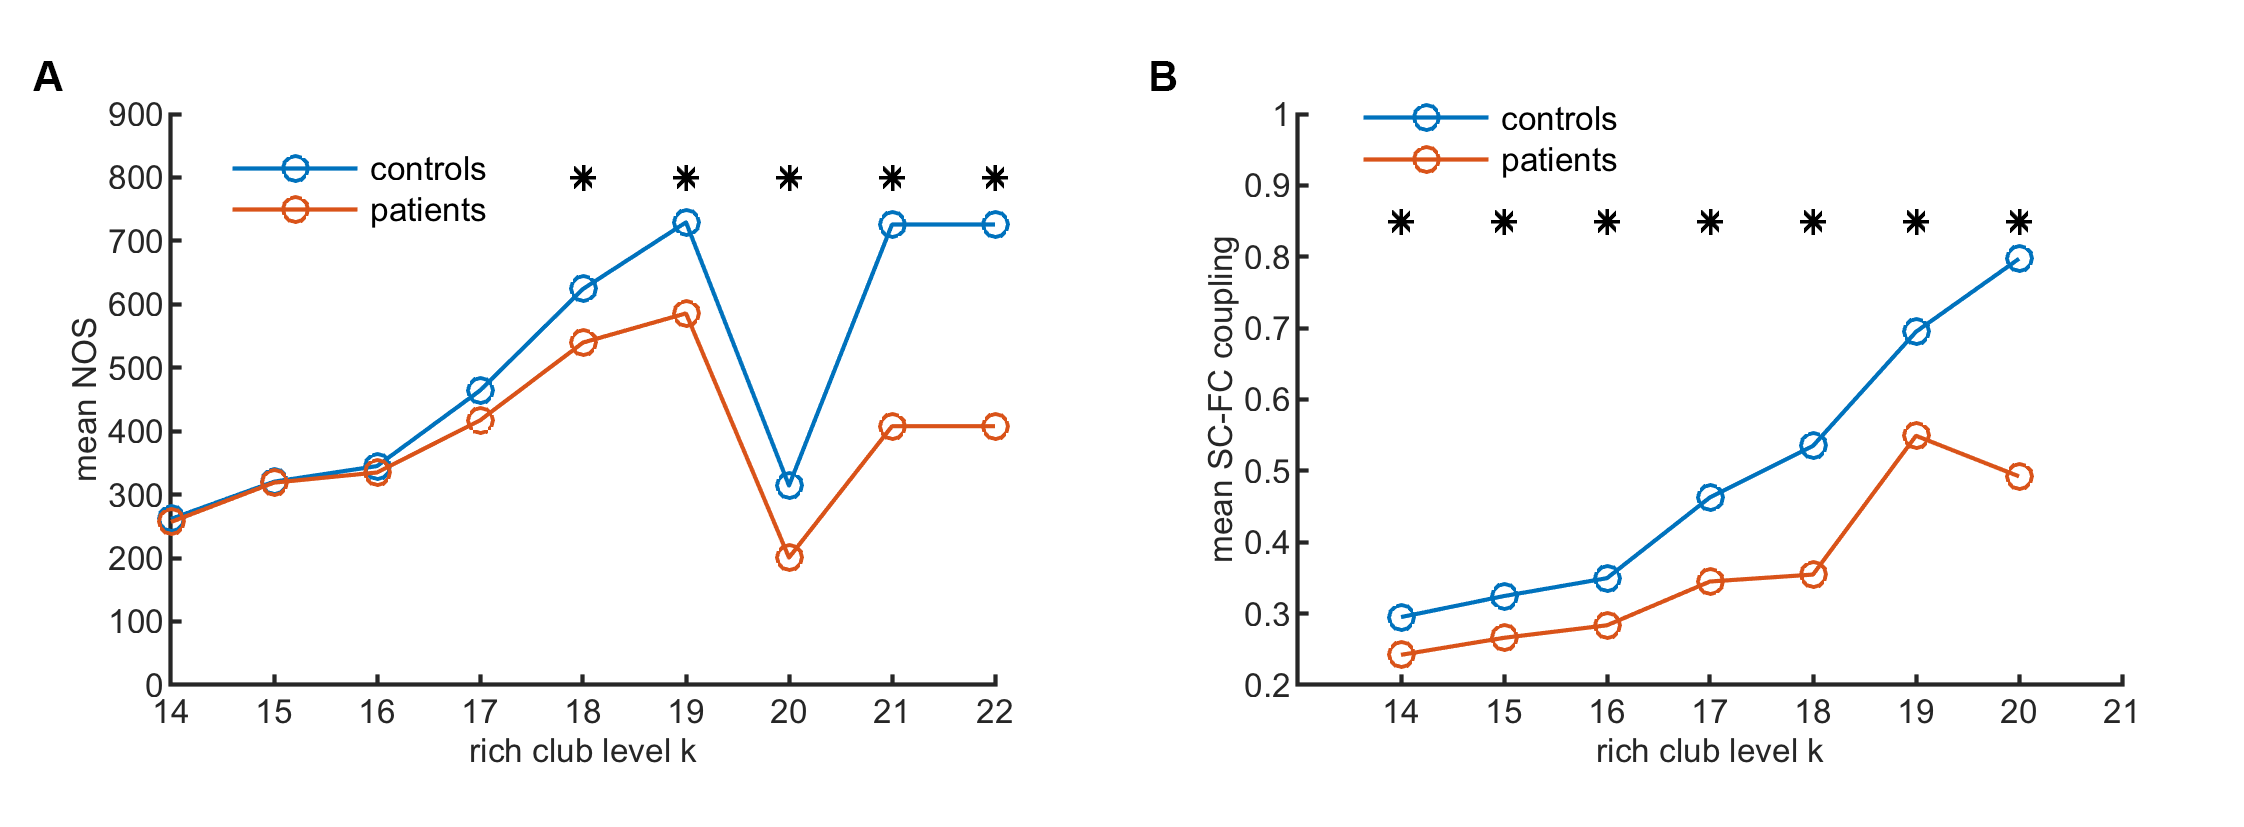
\includegraphics[width=\linewidth]{images/rcsczFigS2.png}
  \caption{\small Rich club alterations in distinct rich club levels. (A) The mean NOS of rich club connections at distinct rich club levels. Patients showed decreased rich club connection weights at k ranged from 18 to 22. (B) The mean SC-FC coupling of rich club connections at distinct rich club levels. Patients showed decreased SC-FC coupling at k ranged from 14 to 20. * indicates effects of \pval < 0.05.
}
  \label{figureS2:range}
\end{figure}

\begin{figure}[H]
\centering
  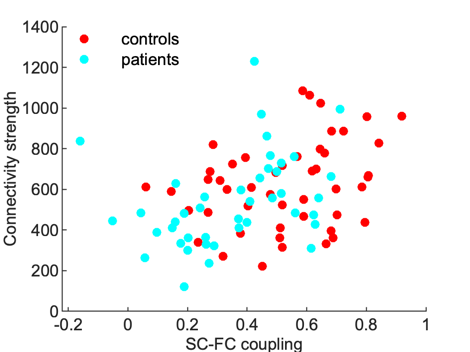
\includegraphics[width=7cm]{images/rcsczFigS3.png}
  \caption{\small Scatter plot of individuals' rich club measurements (in principle dataset). X axis describes SC-FC coupling of rich club connections and Y axis denotes connectivity strength (NOS) of rich club connections.
}
  \label{figureS3:scatter_scfc_nos}
\end{figure}

\begin{figure}[H]
\centering
  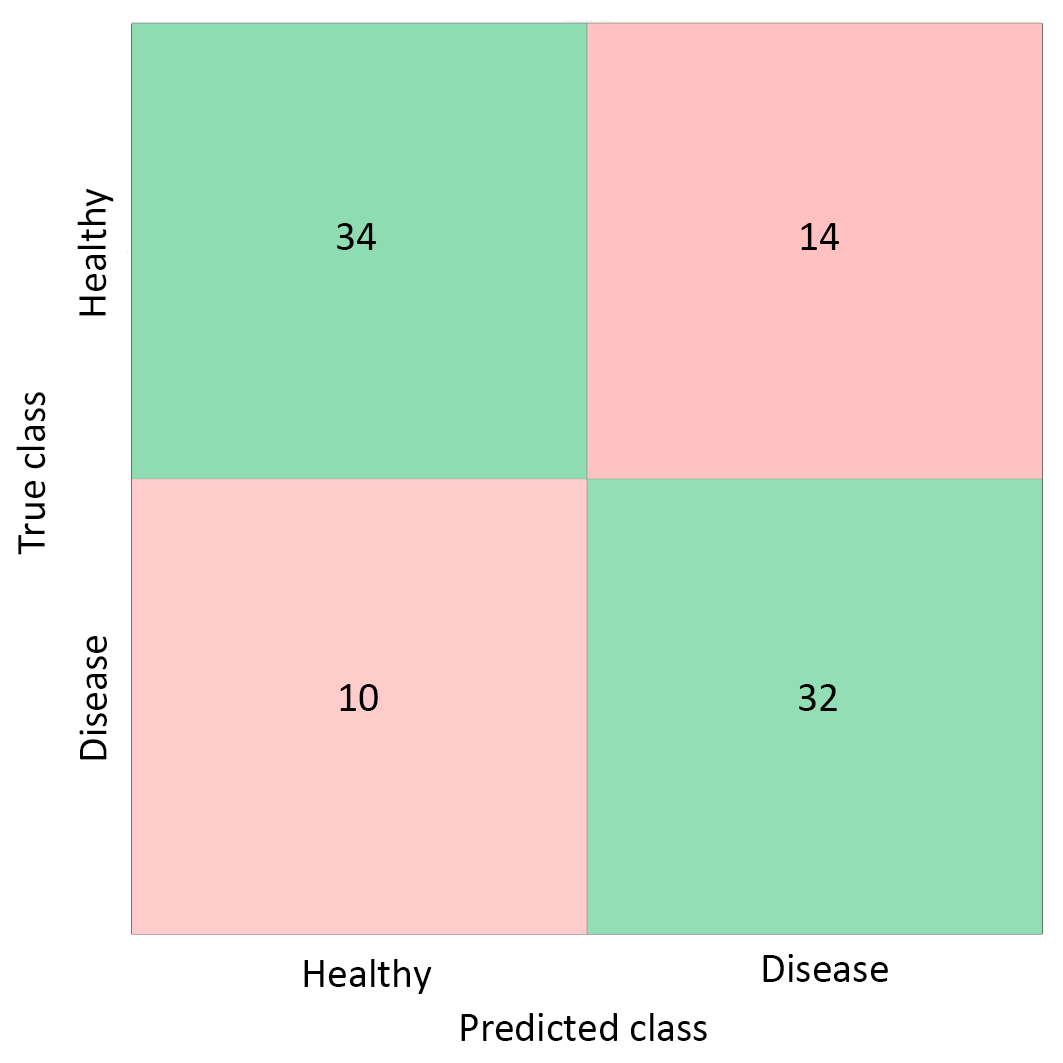
\includegraphics[width=7cm]{images/rcsczFigS4.png}
  \caption{\small Confusion matrix for the machine learning classification. Rows show the true class, and columns show the predicted class. The number of samples in each class are displayed. Green indicates that the true class and predicted class match, otherwise red.
}
\label{figureS4:confusionmatrix}
\end{figure}


\end{refsection}


